\chapter{D3.js and NetFlow}
\label{chp:d3andnetflow} 
\section{Using D3.js}
Earlier in this paper it is mentioned that D3.js will be used to show examples of effective visualization of NetFlow data. It is assumed that the data has already been processed before it is made accessible to these examples. I was supplied with two months of anonymous data from UNINETT to get familiar with NetFlow and be able to use real data for my visualizations. This is anonymized data from January of 2012 from Trondheim and Oslo NetFlow collectors. This means millions of flows.

\subsection{Scope}
The vast amounts of data should be presented with such a scope that is intuitive and easily understandable. Considering NetFlow packages is timestamped and sent from one source address to a specific destination address's port, one will have to chose which of these spectrum's to focus on. In the visual solution it is natural to combine these to represent the data. 

\subsubsection{IP spectrum}
\label{sec:ip_spectrum}
Choosing the address spectrum as the main focus, one will have to find a way to represent the entire IPv4 spectrum. This is alone a challenge, and when it comes to IPv6, it becomes practically impossible. This results in relying more on the pre-processing of the data and segregating the IP-addresses actually worth noticing. In the data provided by UNINETT it is possible to list for example the top 10 files in size, meaning more flows. 
In the data provided by UNINETT this search provided the results in figure \ref{topten}.

\begin{figure}[h!]
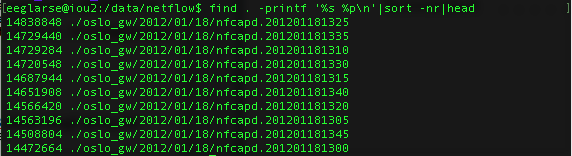
\includegraphics[scale=0.6]{top10}
\caption{Ten files in the provided files with the most flows}
\label{topten}
\end{figure}

From this simple preprocessing it is easy to see that in the time period between 1300-1400 on the 18th of January there was a clear peak in the number of flows having all the spots in the top 10. If we compare to the times with the lowest amount there is a different as they are a fraction of the others.

\begin{figure}
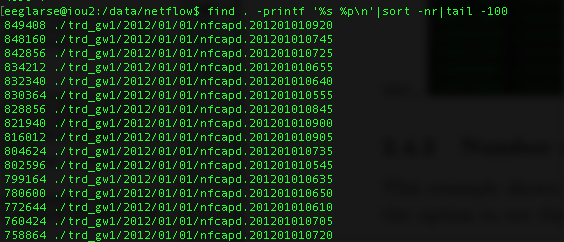
\includegraphics[scale=0.6]{bottom}
\caption{The smallest files from the provided files}
\end{figure}

Trough this we create a .csv file containing the hour in question going further in detail.
Analysing which destination address is the most requested is the next step. 

\begin{figure}
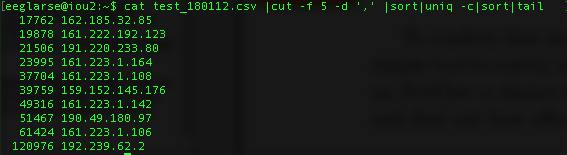
\includegraphics[scale=0.6]{ip_top_list}
\caption{Top ten used destination addresses within the timeframe 1300-1400, 18th of January}
\end{figure}

Again one specific address is clearly separated from the others. At this point we have gotten such into detail on the dataset, it is time to find the reason behind the results we have found. 
These high numbers could be a DDoS attack, or other types of attacks, but not does not necessary ill willed. If we look at the list of top IP-addresses sending packets.

\begin{figure}
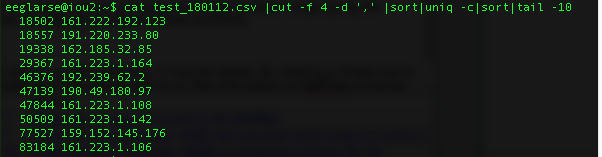
\includegraphics[scale=0.6]{top10_sa}
\caption{Top ten used destination addresses within the timeframe 1300-1400, 18th of January}
\end{figure}

We see that the same IP-address, $192.239.62.2$, is here high up as well. Among hundreds of thousands of addresses in the spectrum. 

To further investigate the activity on certain IP-addresses, it is possible to get the most popular ports on either one specific IP-address, or a list. 
\todo{sjekke opp med portnr og}

\subsubsection{Time spectrum}
On the other side we have the time spectrum. In this case one looks at the amounts of flows within one time slot. Not down to the different IP-addresses. With the vast amount of IP-adresses this is not a suitable spectrum to present the data to find specific attacks etc.. On the other hand it could be used to monitor amounts of traffic over time or which ports are in use at certain times. 

\section{Number of flows to a certain host and port}
\label{sec:d3example}
This example shows how a simple graph can recognize a DDoS attack trough giving the option to see the number of netflows on different hosts and ports. 
\todo{Rette opp}

\subsection{Scope in D3.js}
In this section three modules of a solution is presented to show different levels of detail. It combines both the time spectrum and IP-spectrum to investigate the NetFlow data in different ways. The data from UNINETT required pre-processing before being made available to the D3.js solution. The bash script used can be found in Appendix\ref{chp:appendixb}.

\subsubsection{File structure}
With the bash scripts, thousands of files are created. Data is split into as small and many files as possible to reduce loading time at the user side, and to make sure the data is as comprehensible as possible. In section \ref{sec:atentive} we described the importance of pre-processing the data to highlight certain aspects of larger data sets. With these scripts we perform advanced preprocessing on extreme amounts of data to bring out the desired output to in the best way find deviations.
\todo{Knytte dette opp til preprocessing}

\subsubsection{Overview}
First we have the overview which in this case show an entire year separated into months, weeks and days. 
The purpose of this is to be able to quickly recognize patterns in the data that correlates to periodically activities as backup or launches of new software as mentioned in \ref{patterns}. For example a weekly backup will create similar levels of data usage at specific times each week. 

\begin{figure}[h!]
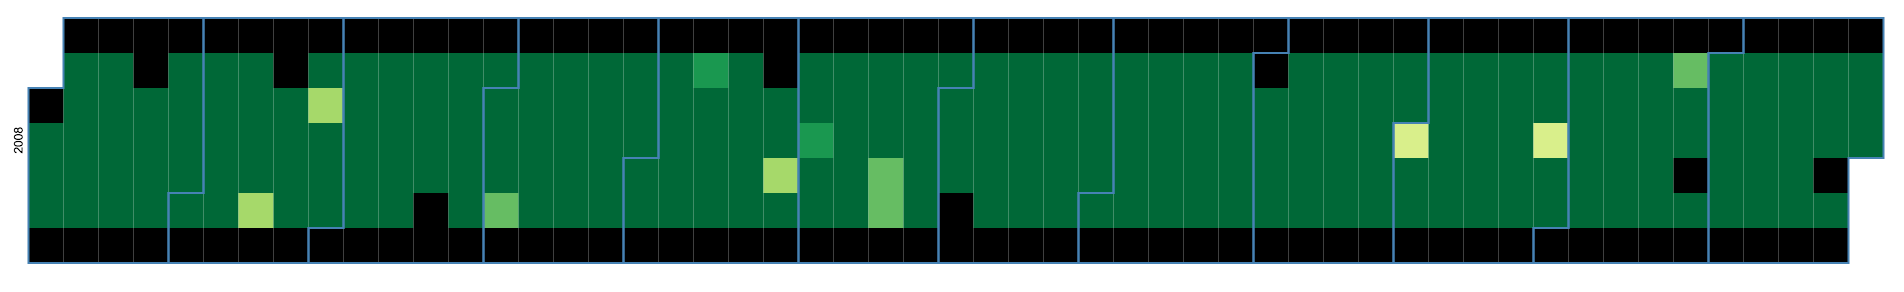
\includegraphics[scale=0.4]{yearly}
\caption{Top ten used destination addresses within the timeframe 1300-1400, 18th of January}
\end{figure}

\subsubsection{IP-addresses and ports}
\label{sec:heatmap}
For each days there are millions of different combinations of which IP-addresses and ports that send flows between each other. Through pre-processing it is possible to distinguish which IP-addresses are the most popular each day, and thus find the ports they use the most. This visualization shows the number of flows for each of these combinations trough a heatmap. A heatmap means it distinguishes values trough a color range based on the highest values in the data set.

\begin{figure}[h!]
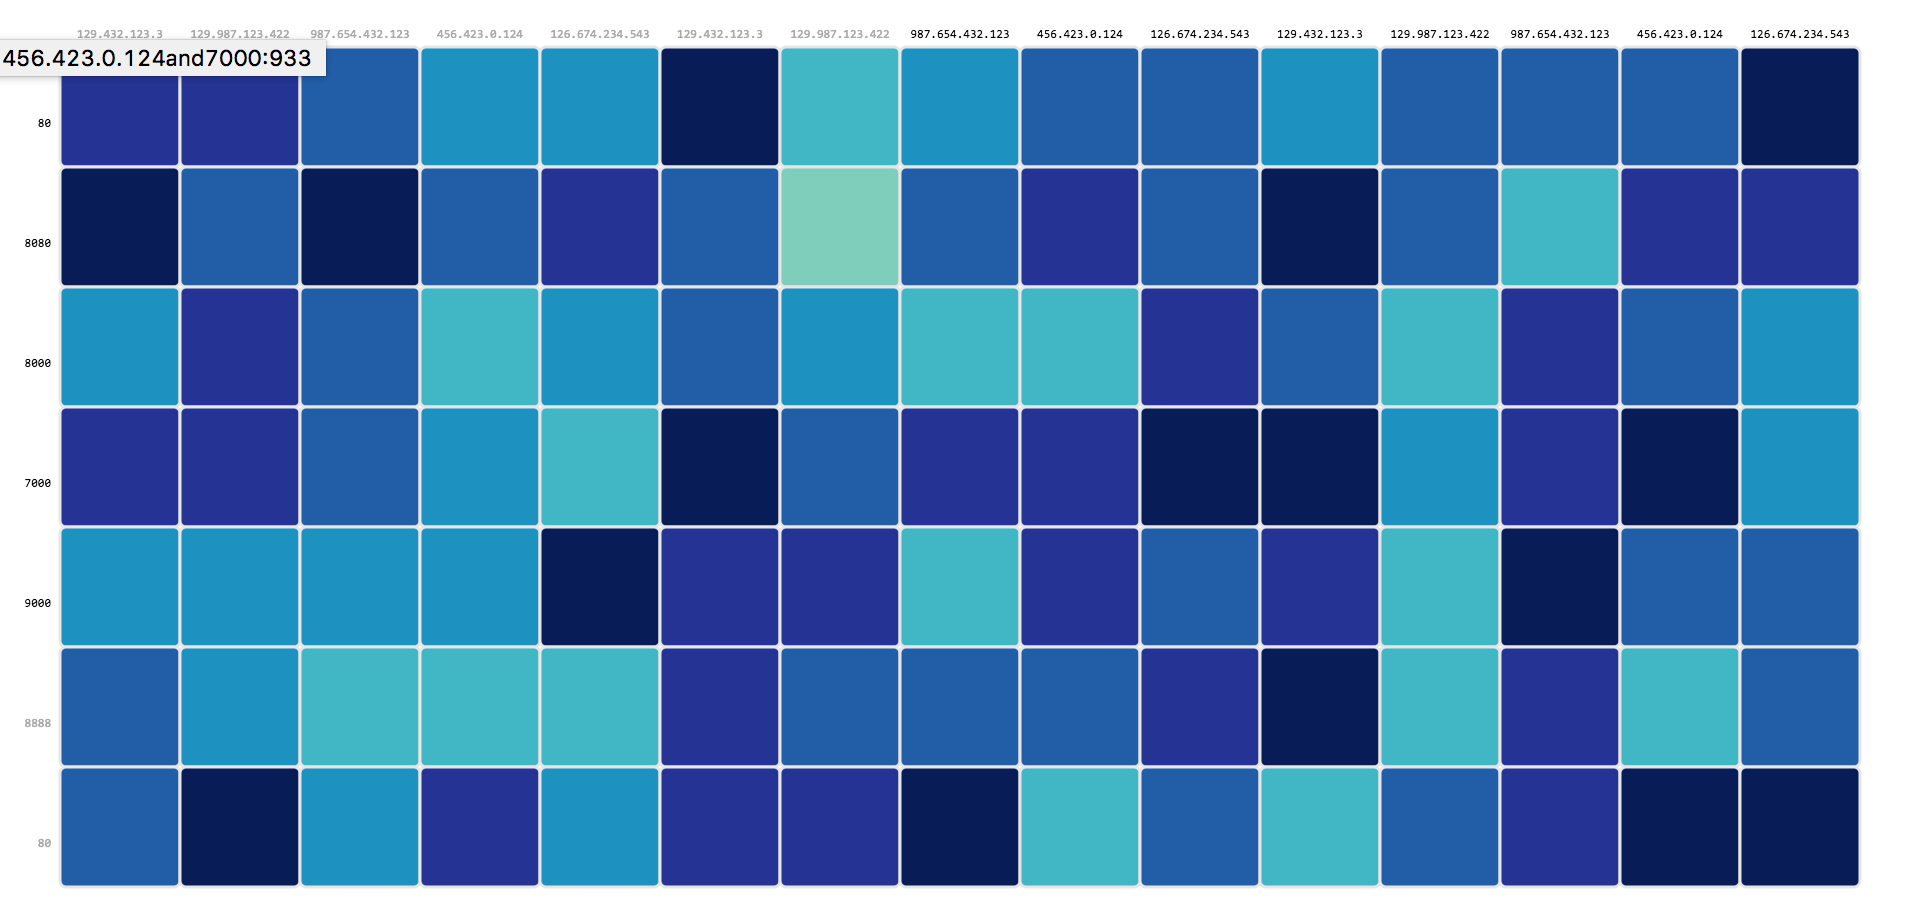
\includegraphics[scale=0.35]{ip_ports}
\caption{Top ten used destination addresses within the timeframe 1300-1400, 18th of January}
\end{figure}

\newpage
\subsubsection{24-hour chart}
When a IP-address and port is selected for a specific day, the next scope is to look at the data in more detail. Using the time-spectrum this graph shows the 24-hour lapse and the amount of flows at each time. 
\begin{figure}[h!]
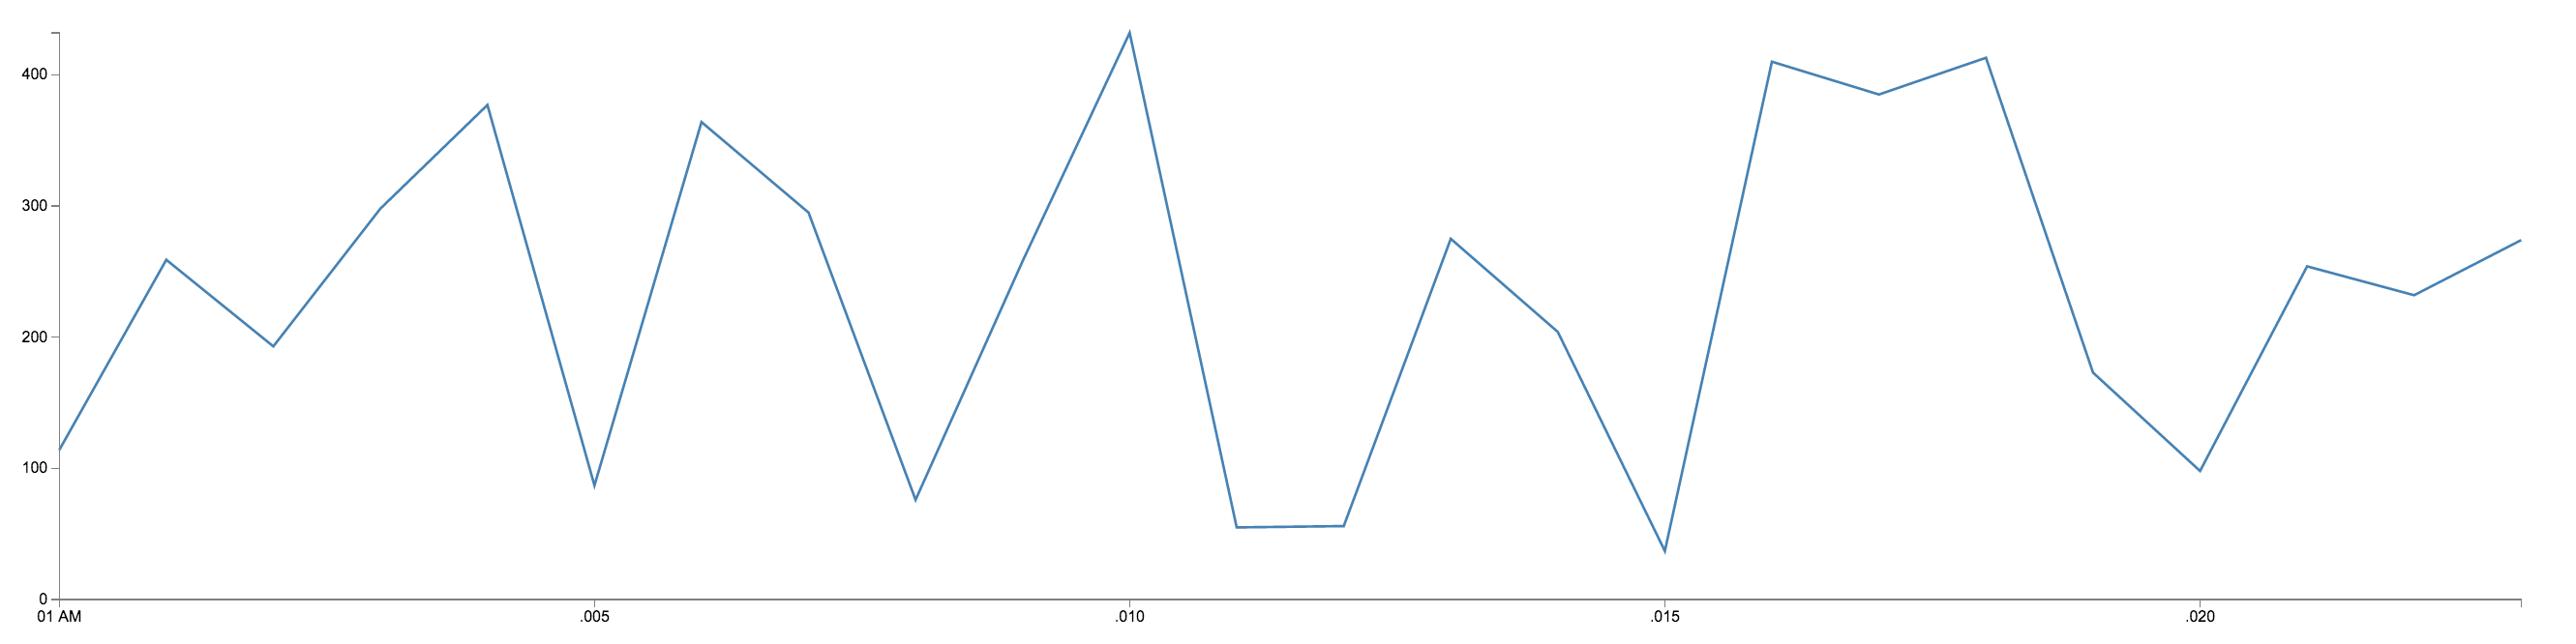
\includegraphics[scale=0.3]{chart}
\caption{Top ten used destination addresses within the timeframe 1300-1400, 18th of January}
\end{figure}
\newpage


\subsection{Pros and cons}
Between the visual solution and the current command line based solution there are pros and cons. Some weighing in more than others depending on the result needed from the solution.
 \todo{refere til noe i background eller en referanse, i pkt 2 av pros for visuell løsning}


\subsubsection{Visual solution}
\begin{table}[h!]
\begin{tabularx}{\linewidth}{>{\parskip1ex}X@{\kern4\tabcolsep}>{\parskip1ex}X}
\toprule
\hfil\bfseries Pros
&
\hfil\bfseries Cons
\\\cmidrule(r{3\tabcolsep}){1-1}\cmidrule(l{-\tabcolsep}){2-2}

%%% PROS, seperated by empty line or \par
Very intuitive and simple to use. Meaning the need for competence within nfdump etc. is not as high, and lowers the threshold to use the tool.

Visual interpretation of data is quicker and easier for the human mind to comprehend. Patterns and other aberrations is more likely to be discovered that would not be as visible in a test based solution.

As mentioned in \ref{sec:dpa}, a goal is to show only the data relevant to the user. Meaning the data that is not pertinent the user is never made visible.

&

%% CONS, seperated by empty line or \par
A visual solution might limit the possibilities that exist in an advanced command line based solution. Meaning that a visual element is limited to some extent. Not showing the whole picture. 

\\\bottomrule
\end{tabularx}
\caption{Pros and cons of a visual solution}
\end{table}

\subsubsection{Command line solution}
\begin{table}[h!]
\begin{tabularx}{\linewidth}{>{\parskip1ex}X@{\kern4\tabcolsep}>{\parskip1ex}X}
\toprule
\hfil\bfseries Pros
&
\hfil\bfseries Cons
\\\cmidrule(r{3\tabcolsep}){1-1}\cmidrule(l{-\tabcolsep}){2-2}

%% PROS, seperated by empty line or \par
A command line solution possess a wide range of very specific commands as in nfdump, providing the possibility to do very distinct searches.

&

%% CONS, seperated by empty line or \par
Such a tool is time consuming and difficult to master. Being very reliable on the searches being correct and providing the exact answer one is looking for requires a fair amount of skill.

Patterns are not easy to recognize when using a command line as it might involve several searches to reveal the information desired. 

\\\bottomrule
\end{tabularx}
\caption{Pros and cons of a command line solution}
\end{table}